%%%%%%%%%%%%%%%%%%%%%%%%%%%%%%%%%%%%%%%%%%%%%%%%%%%%%%%%%%%%%%%%%%%%%%%%%%%%%%%%
% Author : Michaela Mackova, Tomas Polasek (template)
% Description : First exercise in the Introduction to Game Development course.
%   It deals with an analysis of a selected title from the point of its genre, 
%   style, and mechanics.
%%%%%%%%%%%%%%%%%%%%%%%%%%%%%%%%%%%%%%%%%%%%%%%%%%%%%%%%%%%%%%%%%%%%%%%%%%%%%%%%

\documentclass[a4paper,10pt,english]{article}

\usepackage[left=2.50cm,right=2.50cm,top=1.50cm,bottom=2.50cm]{geometry}
\usepackage[utf8]{inputenc}
\usepackage{graphicx}
\usepackage{subfigure}
\usepackage{hyperref}
\hypersetup{colorlinks=true, urlcolor=blue}

\newcommand{\ph}[1]{\textit{[#1]}}

\title{%
Analýza mechaniky%
}
\author{%
Michaela Macková (xmacko13)%
}
\date{}

\begin{document}

\maketitle
\thispagestyle{empty}

{%
\large

\begin{itemize}

\item[] \textbf{Název:} Ori and the Blind Forest

\item[] \textbf{Vydáno:} 2015

\item[] \textbf{Autor:} Moon Studios

\item[] \textbf{Hlavní žánr:} RPG plošinovka

\item[] \textbf{Vedlejší žánr:} Logická

\item[] \textbf{Styl:} Kreslená

\end{itemize}

}

\section*{\centering Analýza}

Hra Ori and the Blind Forest je kreslená RPG plošinovka. Tímto fantasy příběhem procházíme jako malé bílé zvířátko jménem Ori, které postupně sbírá různé předměty a nabíjí si energii, díky které může využívat své schopnosti. Tyto schopnosti se dají postupně vylepšovat nasbíranými věcmi a postupem příběhu dostáváme několik nových schopností.

Ori se snaží získat orb a ten poté odnést k umírajícímu stromu, aby jej oživil. V tomto se promítá právě plošinový styl hry, jelikož se přes překážky snažíme dostat z bodu A do bodu B. Dříve zmíněné předměty se nachází po celé mapě a některé předměty je velmi těžké získat. Zde je právě důležitý logický žánr hry, protože pomocí různých hádanek nejenom obstaráváme potřebné předměty pro vylepšování, ale též se přes ně dostáváme dál v příběhu. Pro vyřešení hádanek je někdy potřeba schopností, které jsme v daném okamžiku ještě nedostali (toto platí pouze pro předměty nepotřebné v příběhu). Hádanky v nás vyvolávají dobré pocity, jelikož nás hra odměňuje za naše prozkoumávání celé mapy, nicméně i bez daného prozkoumávání je možné hru dohrát.

Prolínání žánru logické a plošinovky je dost časté a není tomu divu. Do hry to přidává něco nového než jen skákání přes různé plošiny. Ve hraní je to zakombinováno tak, aby se dalo příběhem projít i přes to, že by nám těžké logické hádanky nešly. Zároveň ale vyřešení několika málo netěžkých hádanek je nutné pro pokračování v příběhu.

Kreslený styl hry se perfektně hodí k fantasy příběhu, kterým procházíme. Prostředí bývají velice barevné s přechody do velmi tmavých a smutných částí mapy, pro vytvoření kontrastu mezi pozadím a~Orim. Bílý Ori tím přináší světlo a naději do pochmurných míst. Tím že je vše kresleno, tak hraním hry nám připadá, jako bychom se dívali na animovanou pohádku.

\begin{figure}
  \centering
  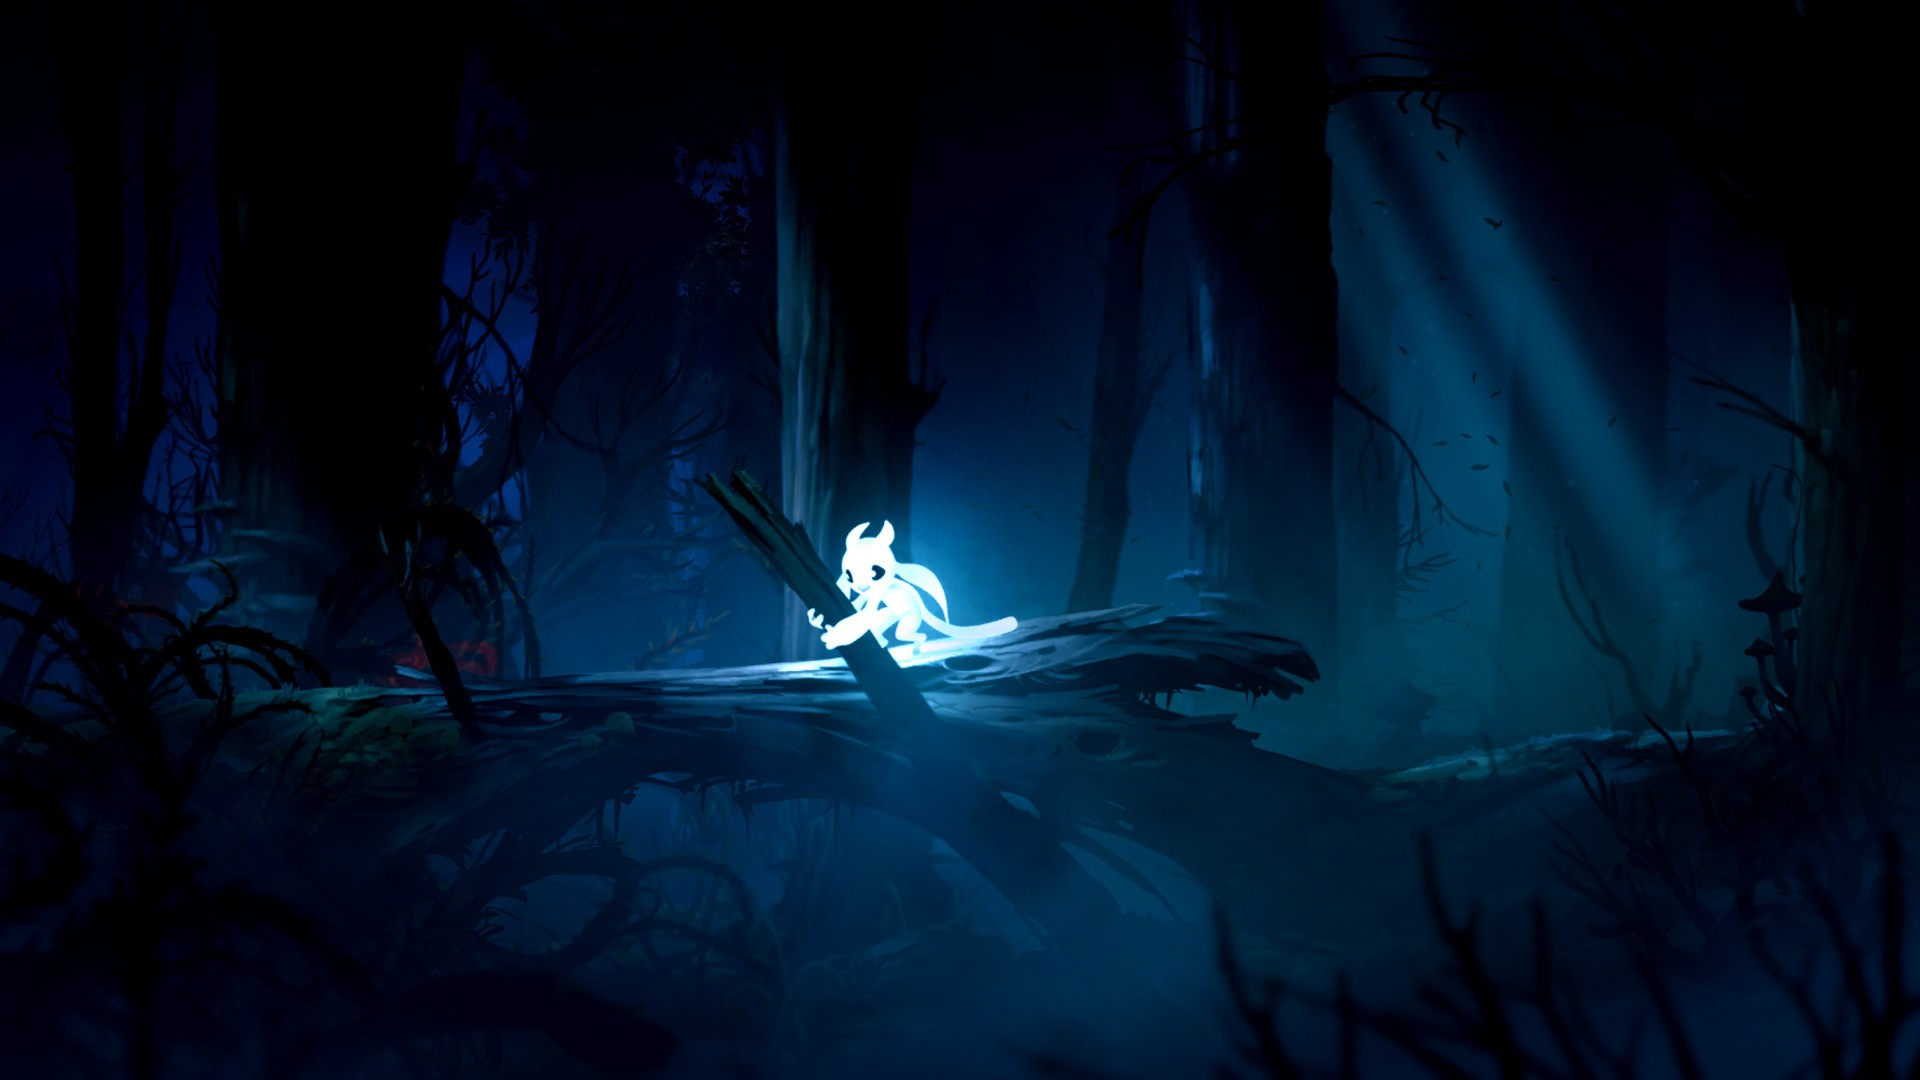
\includegraphics[width=0.49\linewidth]{img/ori_tmave.jpg}
  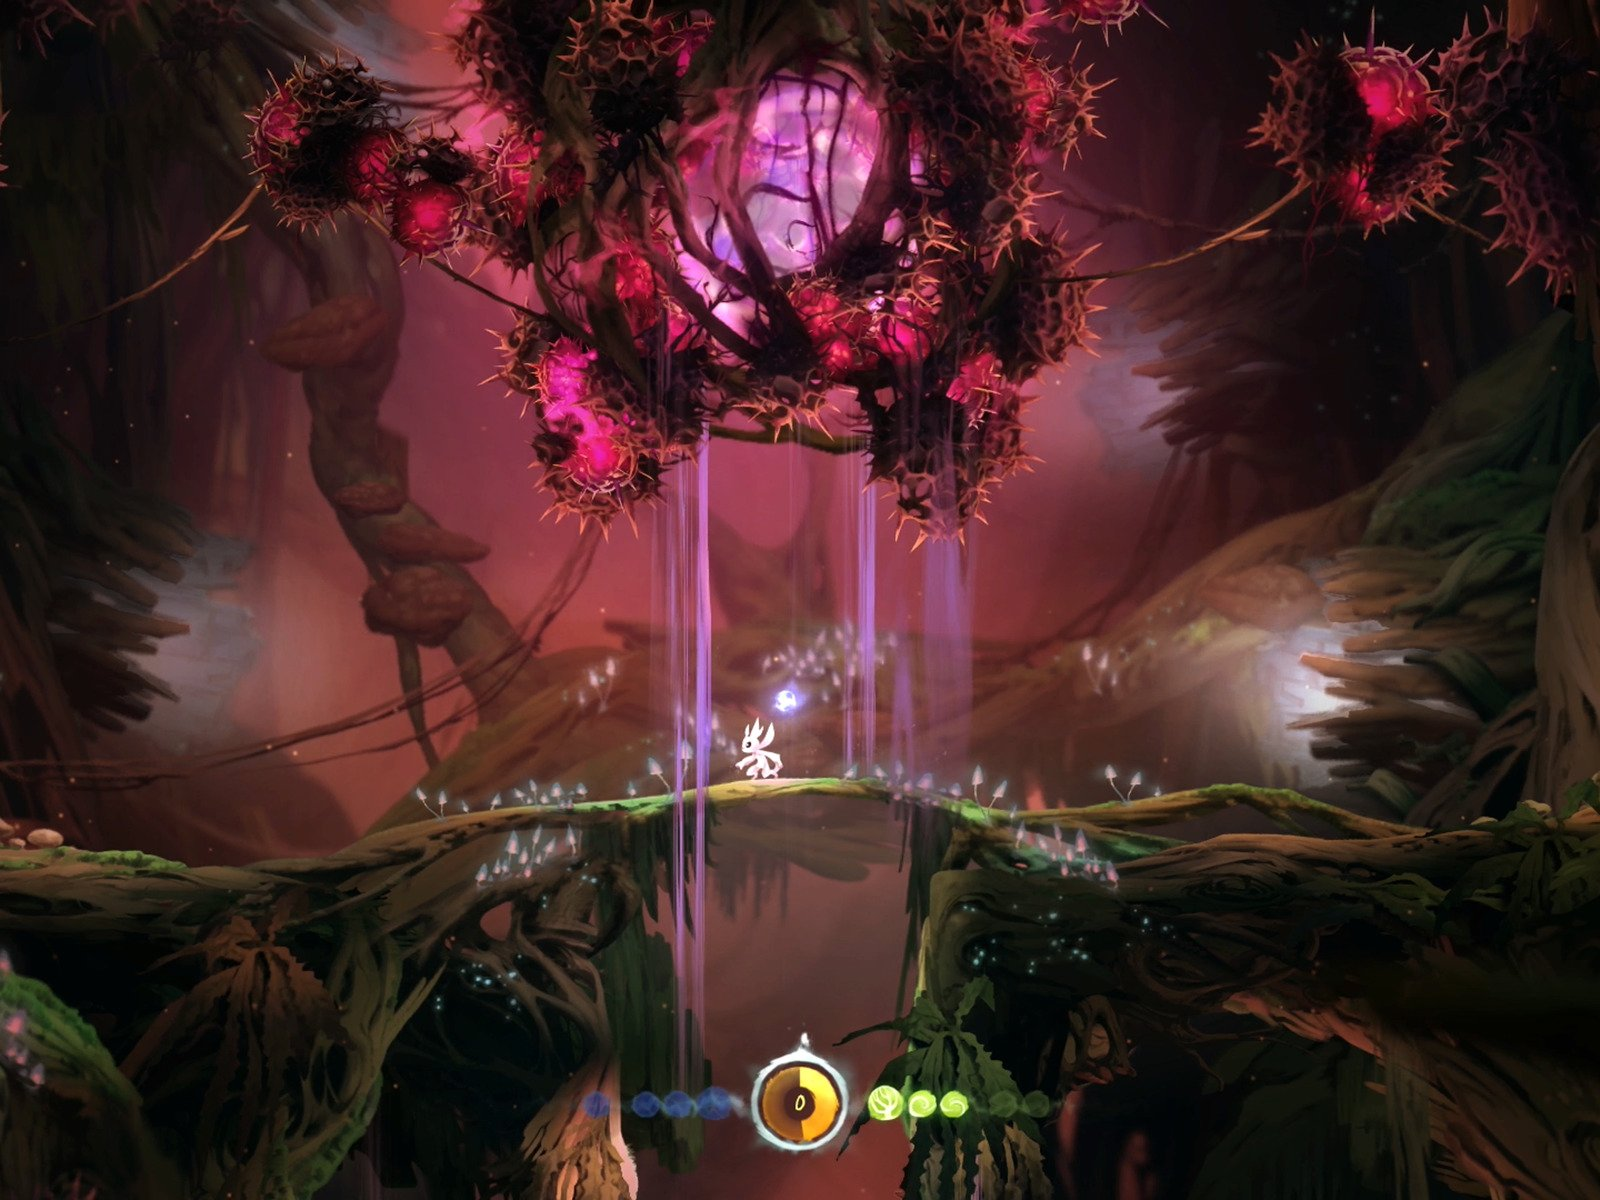
\includegraphics[width=0.49\linewidth]{img/ori.jpg}
\end{figure}

\end{document}
